\documentclass[12pt,a4paper]{article} % Add twocolumn for two-column layout

% Packages
\usepackage[utf8]{inputenc} % UTF-8 encoding
\usepackage[T1]{fontenc}    % Better font encoding
\usepackage{geometry}       % Page layout
\geometry{a4paper, margin=1in}
%% \usepackage{graphicx}       % For images
\usepackage{subcaption}
\usepackage{amsmath, amssymb} % Math symbols
\usepackage{hyperref}       % Hyperlinks
\usepackage{xcolor}         % Text coloring
\usepackage{enumitem}       % Custom lists
\usepackage{caption}        % Captions for figures and tables
\usepackage{booktabs}       % Nicer tables
\usepackage{fancyhdr}       % Custom headers and footers
\usepackage{titlesec}       % Custom section formatting
\usepackage{multicol}       % Multicolumn support
\usepackage{csvsimple}      % Table support
\usepackage{pgfplotstable}
\usepackage{rotating}       % For rotating the table
\usepackage{listings}       % Code blocks


%% \usepackage{showframe}     % Debug

% Custom Header/Footer
\pagestyle{fancy}
\fancyhf{}
\fancyhead[C]{BI-PST Homework}
\fancyfoot[C]{\thepage}

\newcommand{\randv}[2][X]{#1_{\text{#2}}}
\newcommand{\E}{\mathbb{E}}
\newcommand{\var}{\text{var}}

% Section Formatting
\titleformat{\section}{\large\bfseries}{\thesection}{1em}{}
\titleformat{\subsection}{\normalsize\bfseries}{\thesubsection}{1em}{}

% Title Information
\title{BI-PST/24-25 Homework}
\author{Oleksandr Slyvka\\ slyvkole@cvut.cz  \and Illia Lyhin  \\ lyhinill@cvut.cz \and Maksym Khavil \\ khavimak@cvut.cz }
\date{\today} % Can replace with a fixed date or leave blank

\pgfplotstableread[col sep=comma]{./data/case0202.csv}\datatable

\begin{document}
% Title Page
\maketitle
\begin{abstract}
With this document we present homework for BI-PST. Oleksandr Slyvka was chosen as a represntative for our group. He was born 14.04.2006, so we get $K=14$ and $L=6$, then $M = 4$. Such value of $M$ corresponds to case0202 Sleuth dataset, volume of hippocampus with respect to schizofrenia. We will analyse this dataset using numpy, pandas, matplotlib and scipy.stats Python modules.
\end{abstract}
\vspace{1em}

% Sections
\section{Data and estimating moments}

\begin{multicols}{2}

  Firstly, we will load data and display it as a table. There are $n=15$ samples in both categories, values seem to be greater than $1 \text{cm}^3$ and peak arounf $2 \text{cm}^3$, each row repesent a pair of twins, one of whom was affected by schizophrenia.
\columnbreak

\pgfplotstableread[col sep=comma]{./data/case0202.csv}\datatable

  \csvautotabular{./data/case0202.csv} % Auto-generates a table from the CSV
%  \caption{case0202}
%  \label{tab:case0202}

\end{multicols}
\pagebreak

\subsection{Estimations}
  Let $\randv{unaff}$ and $\randv{aff}$ denote random variables of hippocampues volume of those who are unaffected and affected by schizofrenia respectively. Then we will compute estimates of mean, median and variance of those random variables. Median estimation will be chosen as 7th value of sorted sequence of data points. Estimated mean and variance will be computed with following formulas:

\begin{align*}
  \widehat{\E\randv{}} &= m_1 = \bar{X} = \frac{1}{n} \sum_{k = 1}^{n}X_i\\
  \widehat{\var\randv{}} &= s^2 = \frac{1}{n - 1} \sum_{k = 1}^n(X_i - \bar{X})^2
\end{align*}

  Additionaly we will compute uncorrected variance.

\begin{equation*}
  S^2 = \frac{1}{n} \sum_{k = 1}^n(X_i - \bar{X})^2
\end{equation*}

  All those computations are incapsulated in function estimate.

\begin{lstlisting}[basicstyle=\scriptsize]
def estimate(X):
    print(f'{'Mean:' :<30}{X.mean():.3f}')
    print(f'{'Median:' :<30}{X.median():.3f}')
    print(f'{'Variance without correction:' :<30}{((X - X.mean()) ** 2).sum() / n :.3f}')
    print(f'{'Variance with correction:' :<30}{((X - X.mean()) ** 2).sum() / (n - 1):.3f}')
\end{lstlisting}

  After plugging values in we obtain such results.

\begin{align*}
  \widehat{\E\randv{unaff}} &= 1.759 & \widehat{\E\randv{aff}} &= 1.560 \\
  \widehat{F^{-1}_{\randv{unaff}}(0.5)} &= 1.770 & \widehat{F^{-1}_{\randv{aff}}(0.5)} &= 1.590 \\
  \widehat{\var\randv{unaff}} &= 0.059 & \widehat{\var\randv{aff}} &= 0.091 \\
  S^2_{\text{unaff}} &= 0.055 & S^2_{\text{aff}} &= 0.085
\end{align*}

Let's notice that estimated expected value of unaffected distribution is greater than estimated expected value of affected distribution.

\pagebreak
\section{Histograms and empirical cumulitive distribution functions}

We will plot histograms, bins' width will be $0.2 \text{cm}^3$. Near them we will plot empirical cumuitive distribution functions, that will have a step of $1/n$ at each sample value.

Let's plot histogram and ecdf for distribution of unaffected twins.

\begin{figure}[h]
  \centering
  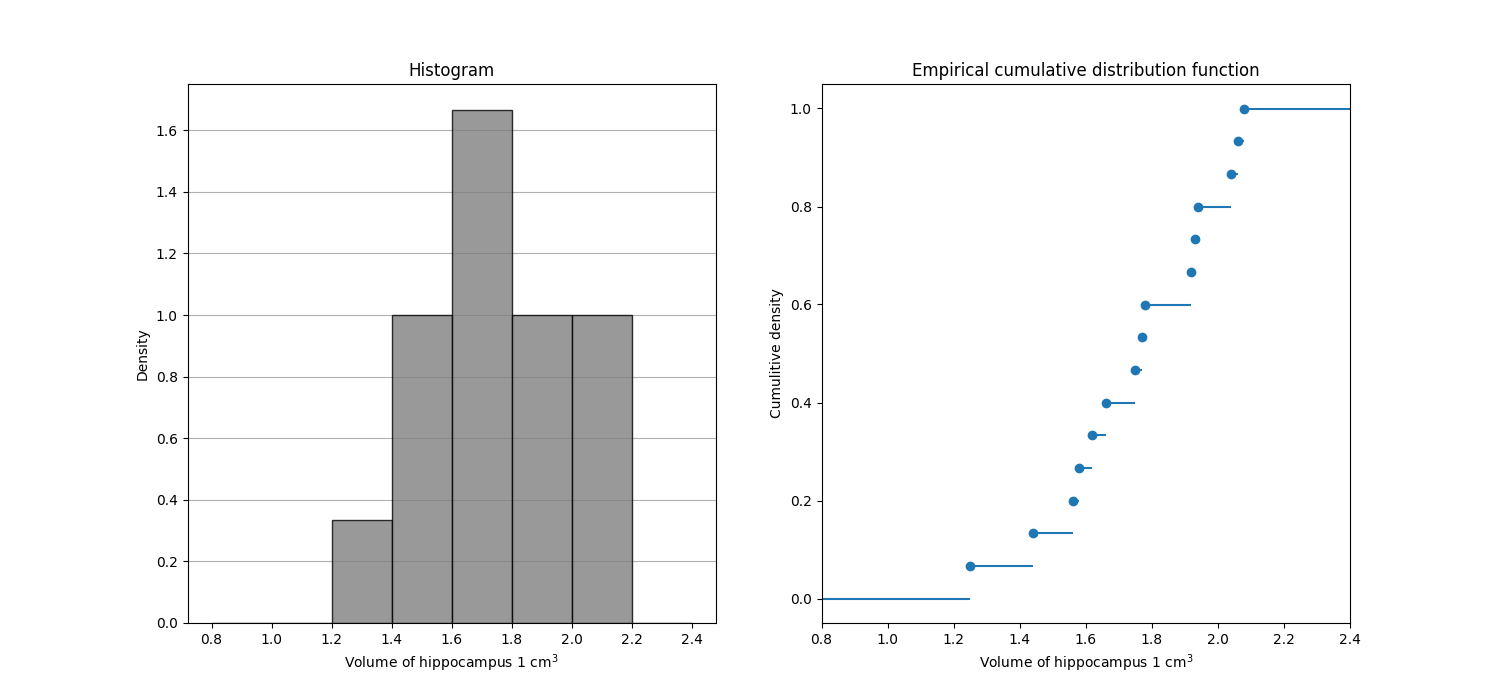
\includegraphics[scale=0.4]{./img/unaffected_hist_ecdf.png}
  \label{fig:unaff_ecdf}
\end{figure}

Here is the same plot for distibution of schizophrenic twins.
\begin{figure}[h]
  \centering
  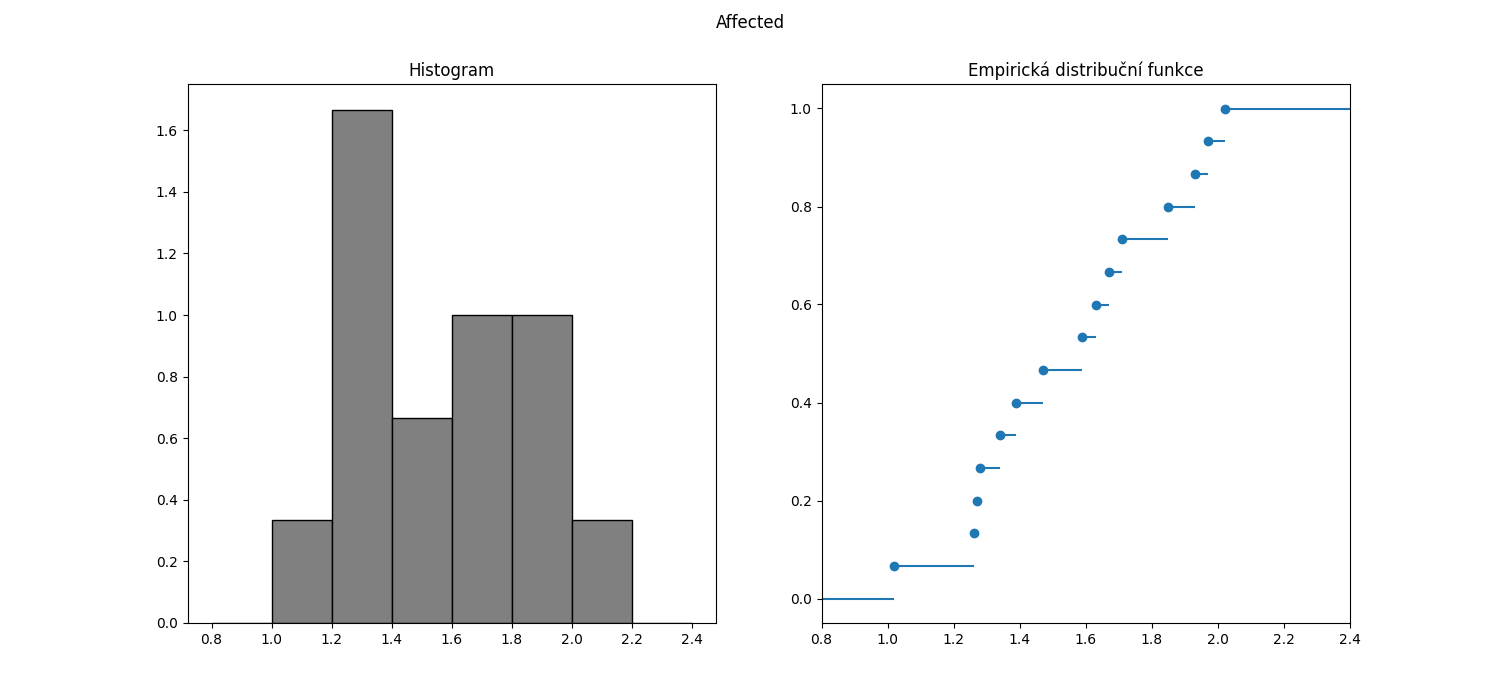
\includegraphics[scale=0.4]{./img/affected_hist_ecdf.png}
  \label{fig:aff_ecdf}
\end{figure}

We can see that later histogram is a little wider, that corresponds with its variance being greater than variance of unaffected distributions. Another observation is that it is altogether slightly shifted towards zero.

\section{Choosing between normal, uniform and exponential distributions}
We will try to model our data as one of the distributions listed above. To do that we need to find parameters of distributions, we will calculate them using method of moments. % TODO: insert link to original paper discussing MoM

\subsection{Calculating parameters}

Normal distribution is parametrized by $\mu$ and $\sigma^2$, uniform distribution is parametrized by its lower and upper bounds resp. $a$ and $b$ and exponential one is parametrized by the rate $\lambda$. All of them can be expressed as functions of at least two moments (exponential can be derived using single moment).

\begin{align*}
  \hat \mu &= m_1 \\
  \hat \sigma^2 &= m_2 - m_1^2 \\
  \hat a &= m_1 - \sqrt{3(m_2 - m_1^2)}\\ 
  \hat b &= m_1 + \sqrt{3(m_2 - m_1^2)}\\ 
  \hat \lambda &= \frac{1}{m_1}
\end{align*}

Those computations are calculated in this code:

\begin{lstlisting}
    m1 = X.mean()
    m2 = (X ** 2).mean()
    mu_hat= m1
    sigma2_hat= m2 - m1 ** 2
    lambda_hat = 1 / m1
    a_hat = m1 - np.sqrt(3 * (m2 - m1**2))
    b_hat = m1 + np.sqrt(3 * (m2 - m1**2))
    print(f"Normal: {mu_hat=}, {sigma2_hat=}")
    print(f"Exp: {lambda_hat=}")
    print(f"Uniform: {a_hat=}, {b_hat=}")
\end{lstlisting}

\pagebreak

\subsection{Comparing histogram and probability distribution functions}

\begin{figure}[h!]
\centering
\begin{subfigure}{0.48\textwidth}
  \centering
  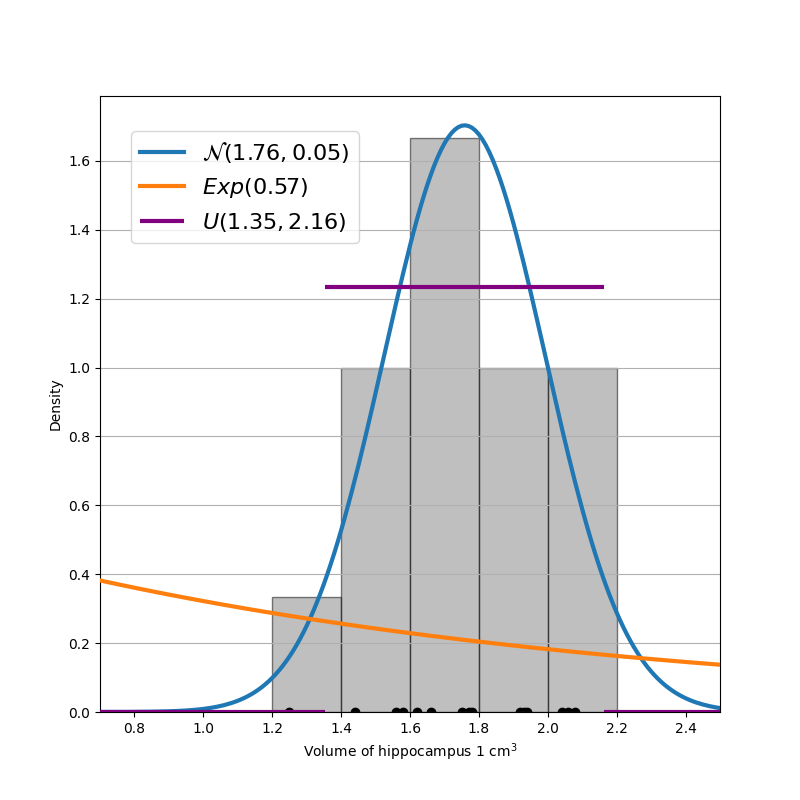
\includegraphics[scale=0.4]{./img/unaffected_distributions.png}
  \label{fig:unaff_dists}
\end{subfigure}
\begin{subfigure}{0.48\textwidth}
  \centering
  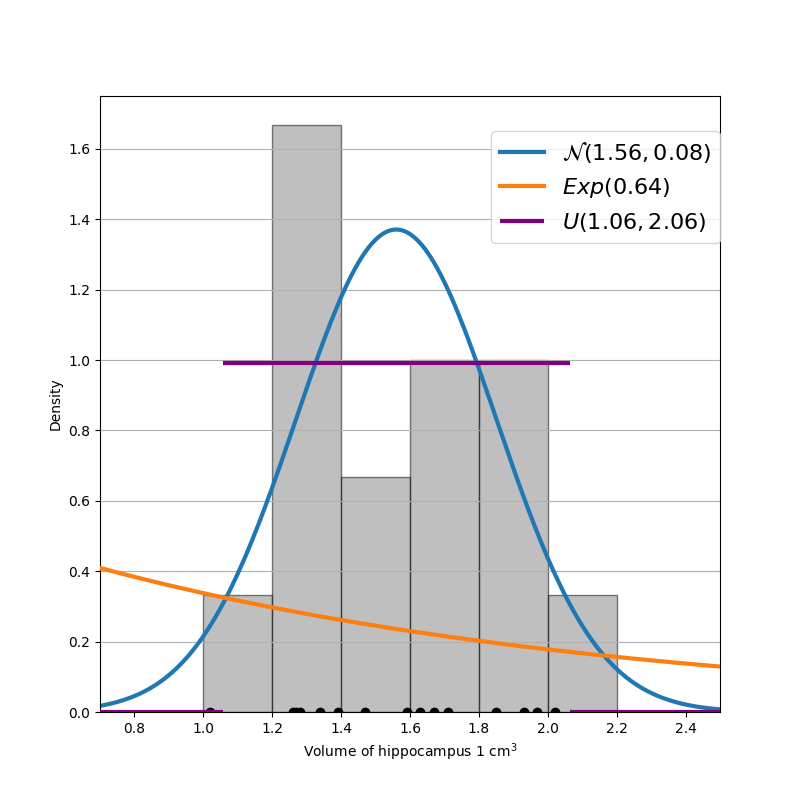
\includegraphics[scale=0.4]{./img/affected_distributions.png}
  \label{fig:aff_dists}
\end{subfigure}
\end{figure}

In both cases exponential distribution performs horribly, so we will reject that immideatly. At both plots there are data points, that lay in zero-probability area for uniform distribution, so it will be rejected too. We are left only with normal distribution, so we naturally choose it, additionaly it matches histogram peaks quite nicely.

\section{Comparing histograms of 100 generated samples and data}

lorem

\section{Computing confidence intervals at $95\%$ level}

lorem

\section{Testing if means equal $K$ at $5\%$ level}

lorem

\section{Testing if means of distributions of volumes affected and unaffected people equal at $5\%$ level}

lorem

% Bibliography (Optional)
\begin{thebibliography}{99}
\bibitem{example} BI-PST 24/25, lectures
\end{thebibliography}

\end{document}
